\section{Appendix}

\begin{figure*}[!ht]
    \centering
    \begin{subfigure}{0.49\textwidth}
        \centering
        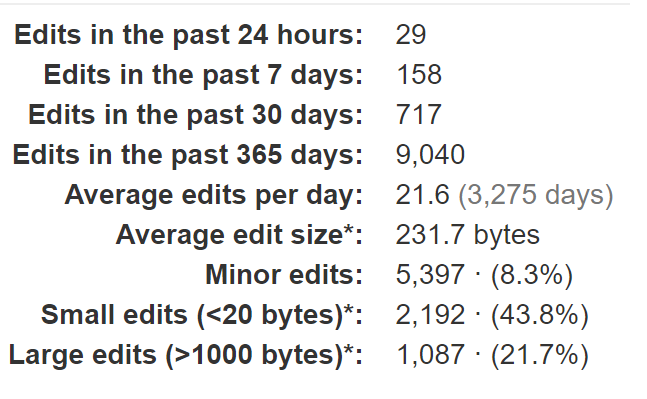
\includegraphics[width=\textwidth]{images/editor_stats.PNG}
        \caption{edit statistics}
        \label{fig:edit-stats}
    \end{subfigure}
    \begin{subfigure}{0.49\textwidth}
        \centering
        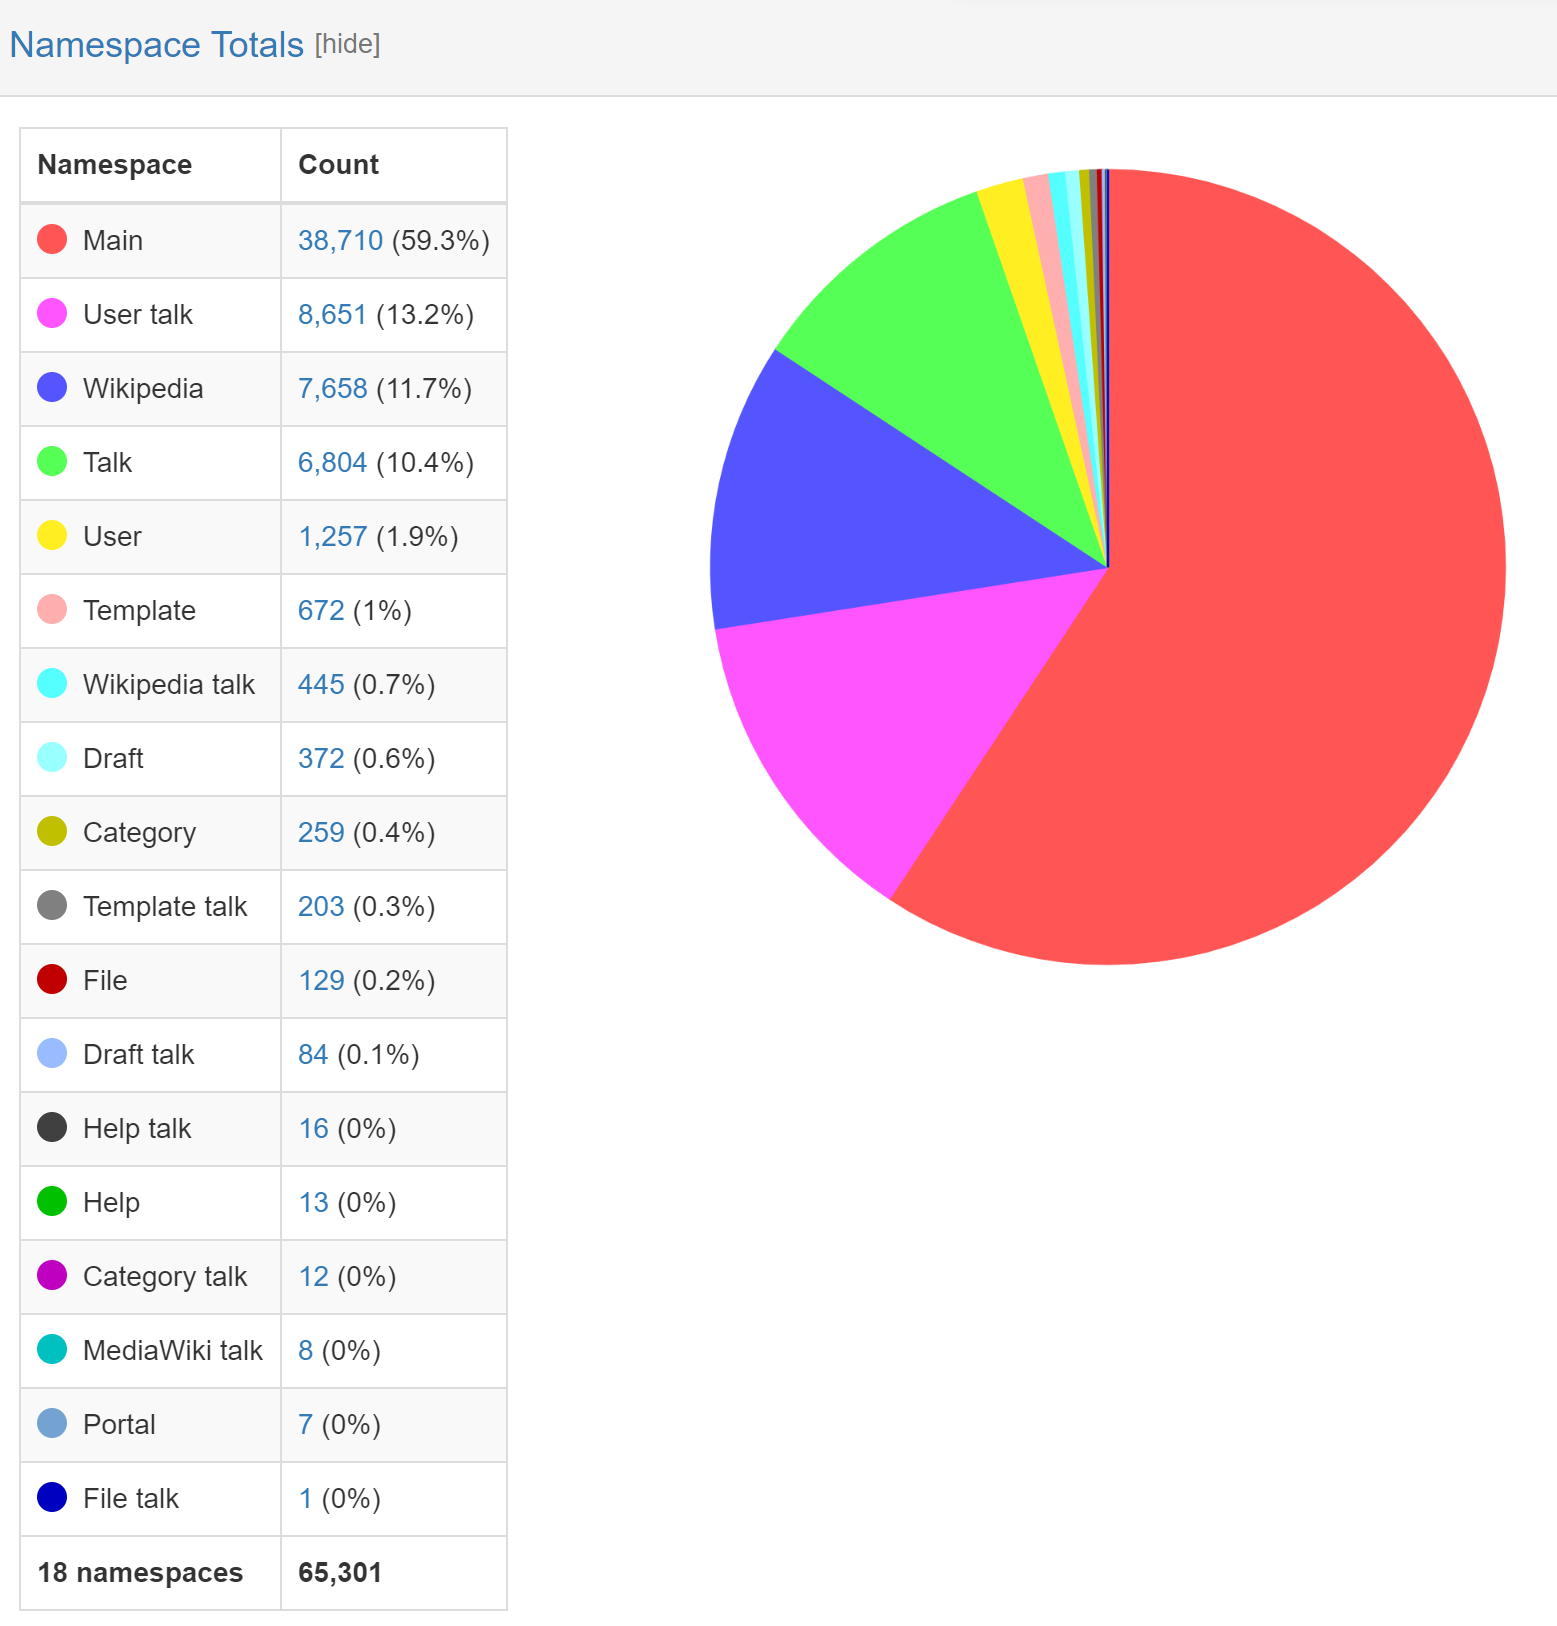
\includegraphics[width=\textwidth]{images/editor_totals.PNG}
        \caption{Edit namespace distribution}
        \label{fig:namespace-totals}
    \end{subfigure}

    \begin{subfigure}{0.49\textwidth}
        \centering
        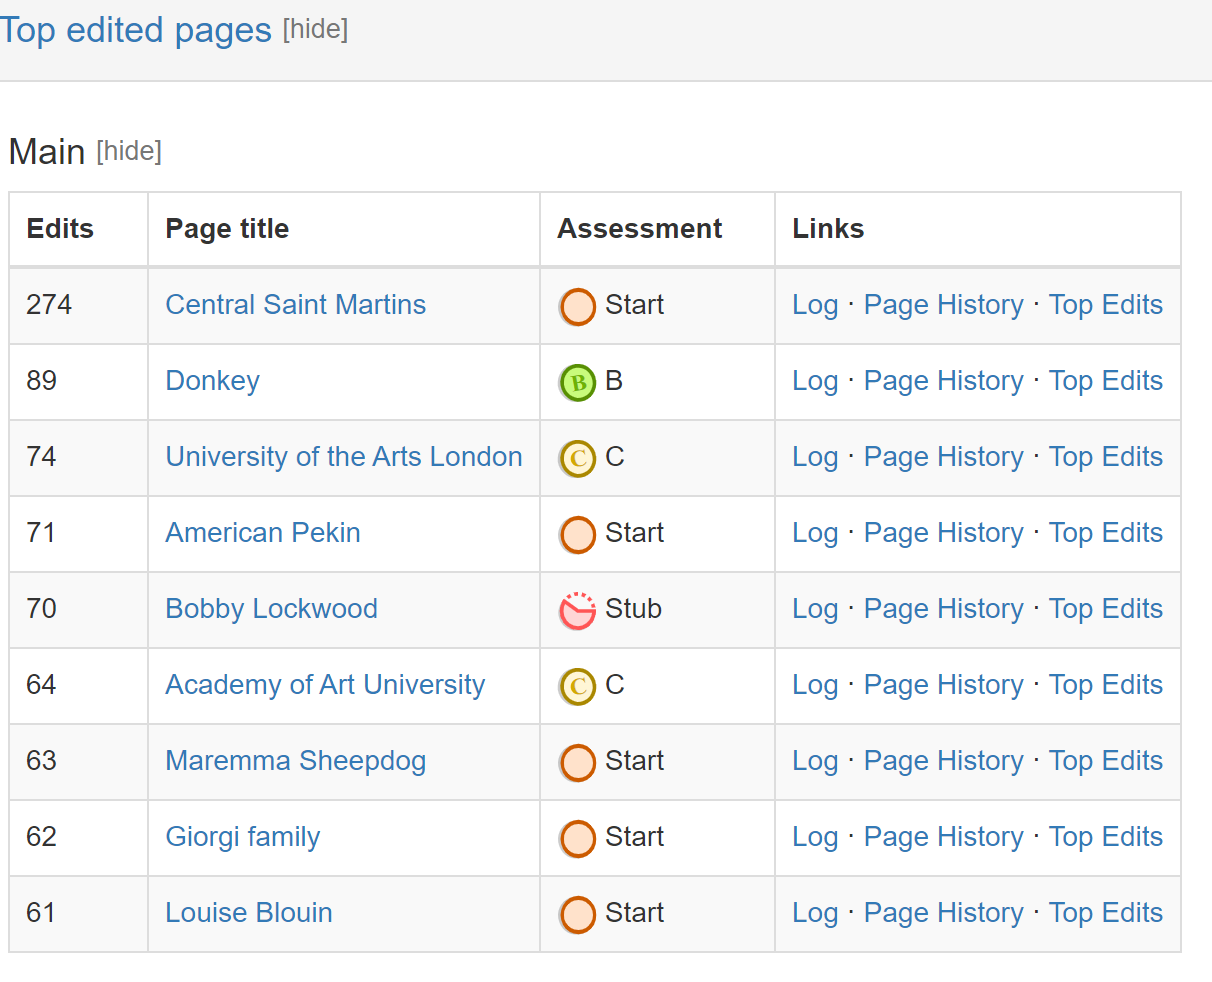
\includegraphics[width=\textwidth]{images/editor_top_edits.PNG}
        \caption{Top edited pages}
        \label{fig:top-edits}
    \end{subfigure}
    \begin{subfigure}{0.49\textwidth}
        \centering
        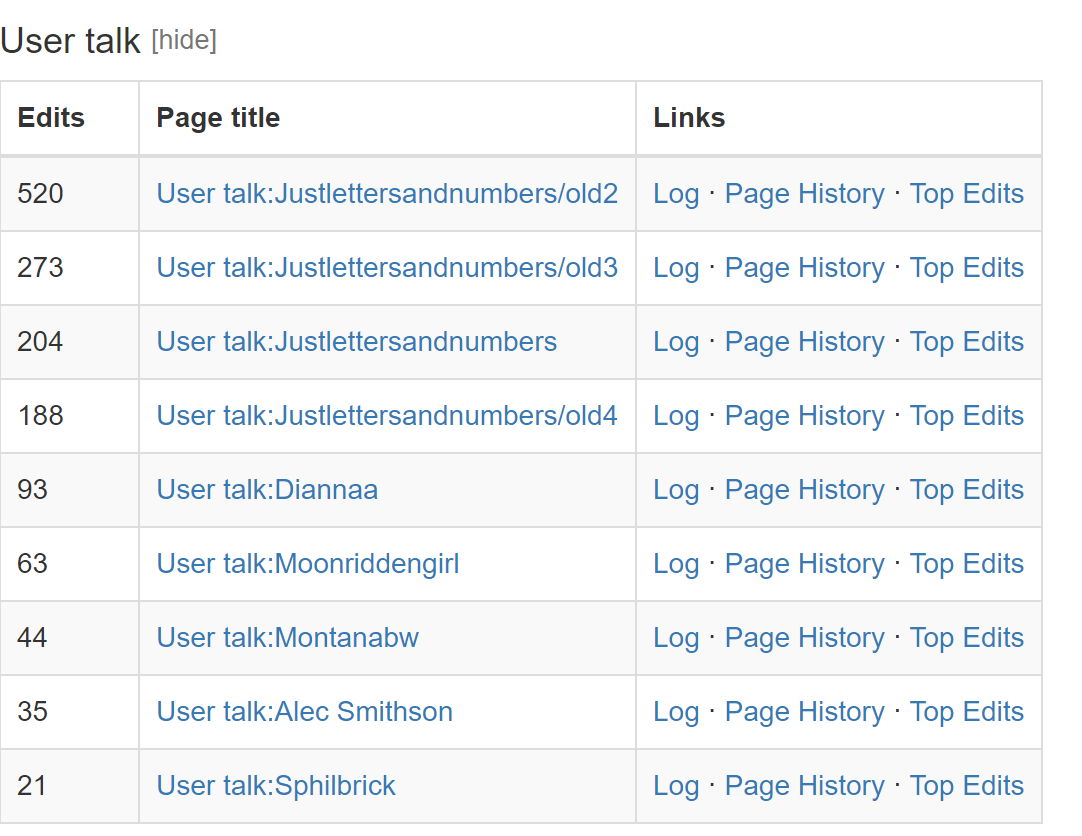
\includegraphics[width=\textwidth]{images/editor_user_talk.PNG}
        \caption{Top user talk pages edits}
        \label{fig:user-talk-edits}
    \end{subfigure}

    \caption{Edit summary of a Wikipedia user}
    \label{fig:edit-summary}
\end{figure*}

\begin{figure*}[!ht]
    \centering
    \begin{subfigure}{0.49\textwidth}
        \centering
        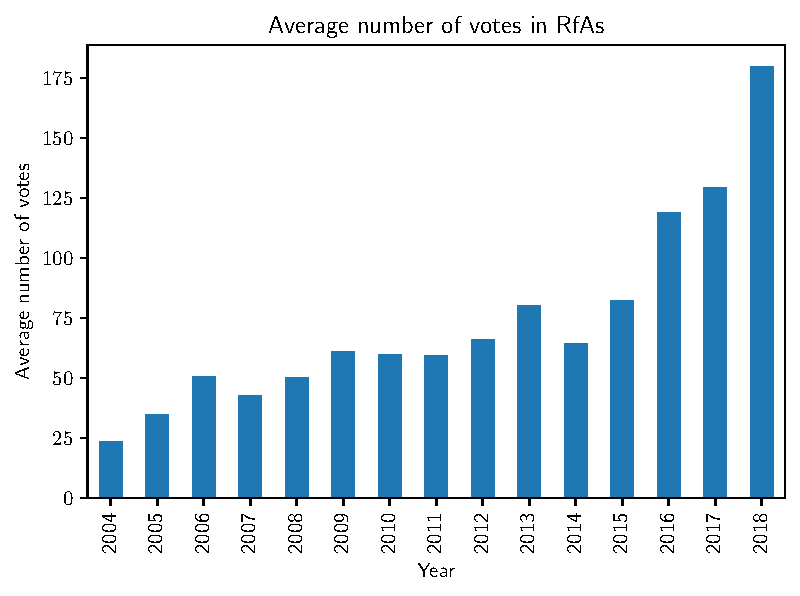
\includegraphics[width=\textwidth]{images/avg_votes.pdf}
        \caption{Vote distribution}
        \label{fig:vot-distribution}
    \end{subfigure}
    \begin{subfigure}{0.49\textwidth}
        \centering
        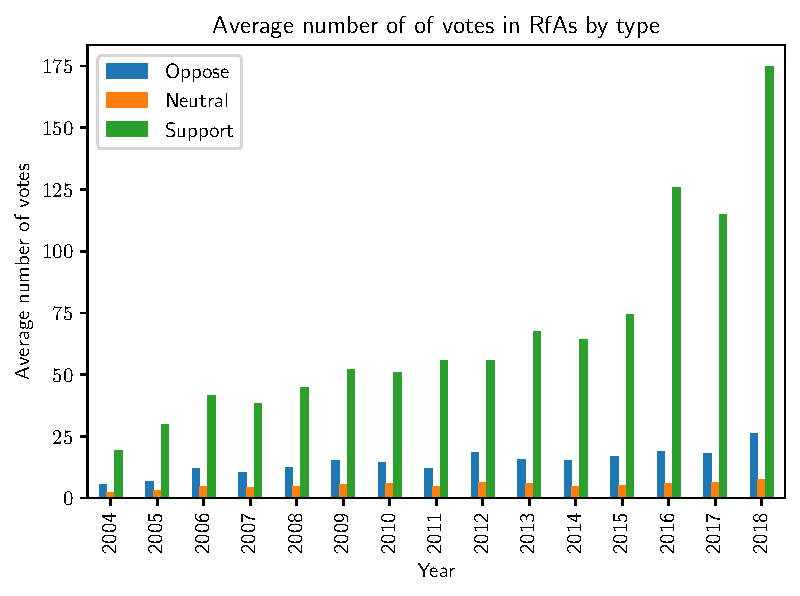
\includegraphics[width=\textwidth]{images/avg_votes_type.pdf}
        \caption{Vote distribution by tye }
        \label{fig:vote-type-distribution}
    \end{subfigure}
    
    \begin{subfigure}{0.49\textwidth}
        \centering
        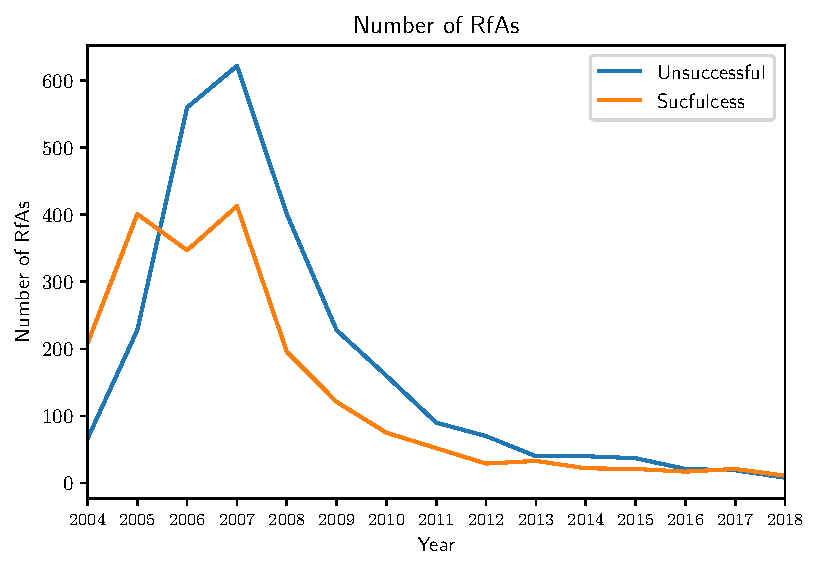
\includegraphics[width=\textwidth]{images/num_rfas.pdf}
        \caption{Number of RfA by year}
        \label{fig:num-rfas}
    \end{subfigure}
    \begin{subfigure}{0.49\textwidth}
        \centering
        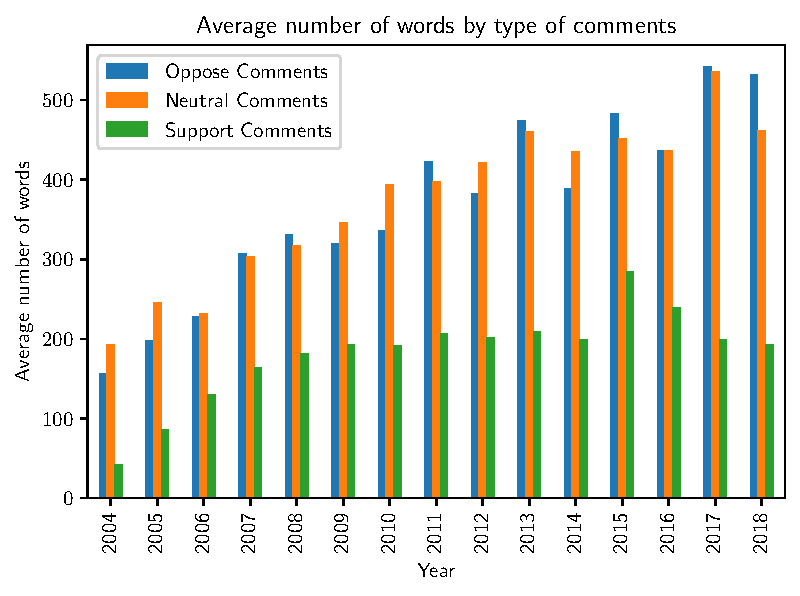
\includegraphics[width=\textwidth]{images/avg_comment_size_type.pdf}
        \caption{Comments distribution}
        \label{fig:comment-distribution}
    \end{subfigure}
    \caption{Election Statistics}
    \label{fig:Election-stats}
\end{figure*}
\clearpage
\begin{figure*}[h!]
    \centering
    \begin{tikzpicture}[remember picture,every
    node/.style={draw,circle,fill=blue,minimum width=4pt}]
        \node (C1) {};
        \node[below=0.7cm of C1]  (C2){};
        \node[right=0.8cm of C1] (C3){};
        \node[right=0.8cm of C2] (C4){};
        \node[below=0.7cm of C4]  (C5){};
        \node[right=0.8cm of C4]  (C6){};
        \draw (C4) -- (C5) -- (C6) -- (C2);
        \draw (C3) -- (C1) -- (C2) -- (C4) -- (C1);
        \draw (C3) -- (C6); 
        \node[draw=none,fill=none,rectangle,above=0.5cm of C1,xshift=-0.5cm,anchor=south west]{Social Graph };
        \path (current bounding box.north east) -- 
        (current bounding box.south east) coordinate[midway] (2BL);
    \end{tikzpicture}
    \hspace*{2.5cm}%
    \begin{tikzpicture}[remember picture,every
    node/.style={draw,circle,fill=red,minimum width=4pt}]
        \node (C1) {};
        \node[below=0.7cm of C1]  (C2){};
        \node[right=0.8cm of C1] (C3){};
        \node[right=0.8cm of C2] (C4){};
        \node[below=0.7cm of C4]  (C5){};
        \node[right=0.8cm of C4]  (C6){};
        \draw[-latex] (C6) -- (C3);
        \draw[-latex] (C1) -- (C2);
        \draw[-latex] (C5) -- (C6);
        \draw[-latex] (C2) -- (C4);
        \path (C4) edge [loop above] (C4); 
        \node[draw=none,fill=none,rectangle,above=0.5cm of C1,xshift=-0.5cm,anchor=south
        west]{Delegation Graph};
        \coordinate[below=2.5cm of C1] (X);
        \draw[white](X)--++(1cm,0);
        \path (current bounding box.north west) -- 
        (current bounding box.south west) coordinate[midway] (2BR);
        \path (current bounding box.south west) -- 
        (current bounding box.south east) coordinate[midway] (2BB);
        \path (current bounding box.south east) -- 
        (current bounding box.north east) coordinate[midway] (2FM);
    \end{tikzpicture}
    \hspace*{3cm}%
    \begin{tikzpicture}[remember picture,every
        node/.style={draw,circle,fill=green,minimum size=1pt}]
        \node[scale=1] (C1) {};
        \node[below=0.7cm of C1,scale=1.75]  (C2){};
        \node[right=0.8cm of C1,scale=2.19] (C3){};
        \node[right=0.8cm of C2,scale=3.5] (C4){};
        \node[below right=0.8cm of C4,scale=1]  (C5){};
        \node[right=0.8cm of C4,scale=1.5]  (C6){};
        \draw[-latex] (C6) -- (C3);
        \draw[-latex] (C1) -- (C2);
        \draw[-latex] (C5) -- (C6);
        \draw[-latex] (C2) -- (C4);
        \path (C4) edge [loop below] (C4); 
        \node[draw=none,fill=none,rectangle,above=0.5cm of C1,xshift=-0.5cm,anchor=south
        west]{Node Importance Graph};
        \coordinate[below=2.5cm of C1] (X);
        \draw[white](X)--++(1cm,0);
        \path (current bounding box.north west) -- 
        (current bounding box.south west) coordinate[midway] (3BU);
        \end{tikzpicture}
        \tikz[overlay,remember picture]{\draw[-latex,thick] (2BL) -- (2BL-|2BR)
        node[midway,above,text width=2.5cm]{Delegation Rule};} 
        \tikz[overlay,remember picture]{\draw[-latex,thick] (2FM) -- (3BU)
        node[midway,above,sloped,text width=2.5cm]{Katz Centrality $\alpha=0.5$};} 
        
        \caption{Viscous Democracy}
        \label{fig:viscous-dem}
    \end{figure*}